\documentclass[../DoAn.tex]{subfiles}
\usepackage{graphicx}
\usepackage[utf8]{inputenc}
\usepackage{float}
\usepackage{subcaption}
\usepackage{array}
\usepackage{subfig}
\usepackage[labelfont=it]{caption}
\usepackage{fancyvrb} % Thay thế listings bằng fancyvrb
\usepackage{xcolor}

% Thiết lập đánh số hình theo chương
\numberwithin{figure}{chapter}

\captionsetup[subfigure]{
    labelfont=it,
    labelformat=simple,
    labelsep=space
}

\renewcommand{\thesubfigure}{Hình \thefigure.\arabic{subfigure}}

\begin{document}

Dart, một ngôn ngữ lập trình đa năng do Google phát triển, đã chuyển mình từ một ứng cử viên thay thế JavaScript thành một trụ cột quan trọng trong phát triển ứng dụng đa nền tảng hiện đại. Được công bố rộng rãi vào năm 2011, Dart giờ đây hỗ trợ các ứng dụng trên web, di động, máy tính để bàn và phía máy chủ, nhờ vào sự kết hợp với Flutter cùng bộ tính năng mạnh mẽ. Phần này sẽ giới thiệu nguồn gốc, các mốc phát triển quan trọng và vai trò của Dart trong việc giúp các nhà phát triển tạo ra ứng dụng đa nền tảng hiệu suất cao từ một mã nguồn duy nhất.

\begin{figure}[H]
    \centering
    
\includegraphics[width=0.5\textwidth]{Hinhve/dartimg.png}
    \caption{Ngôn ngữ lập trình Dart}
    \label{fig:dartimg}
\end{figure}

\section{Giới thiệu về ngôn ngữ Dart}
\subsection{Hoàn cảnh ra đời của ngôn ngữ lập trình Dart}

Dart là một ngôn ngữ lập trình được Google giới thiệu nhằm khắc phục những hạn chế của JavaScript trong việc xây dựng các ứng dụng web lớn, đặc biệt về hiệu suất và khả năng bảo trì. Để hiện thực hóa mục tiêu này, Google đã giao cho hai kỹ sư Lars Bak và Kasper Lund phát triển Dart, và ngôn ngữ này chính thức được công bố tại hội nghị GOTO ở Aarhus, Đan Mạch, vào ngày 10 tháng 10 năm 2011. Sự kiện ra mắt này đánh dấu bước tiến quan trọng trong việc cung cấp một công cụ lập trình hiện đại, dễ học và có hiệu suất cao. Đặc biệt, Dart được thiết kế để có thể biên dịch sang JavaScript, giúp đảm bảo tính tương thích với các trình duyệt web phổ biến, đồng thời hỗ trợ phát triển ứng dụng trên nhiều nền tảng khác nhau như web, di động và máy tính.


\begin{figure}[H]
    \centering
    \begin{subfigure}[b]{0.35\textwidth}
        \centering
        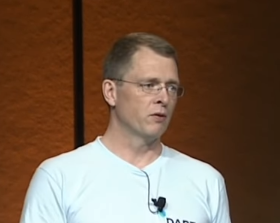
\includegraphics[width=\textwidth,height=3.5cm,keepaspectratio]{Hinhve/Lars_Bak.png}
        \caption{Lars Bak}
        \label{subfig:lars_bak}
    \end{subfigure}%
    \hspace{0.5cm} 
    \begin{subfigure}[b]{0.42\textwidth}
        \centering
        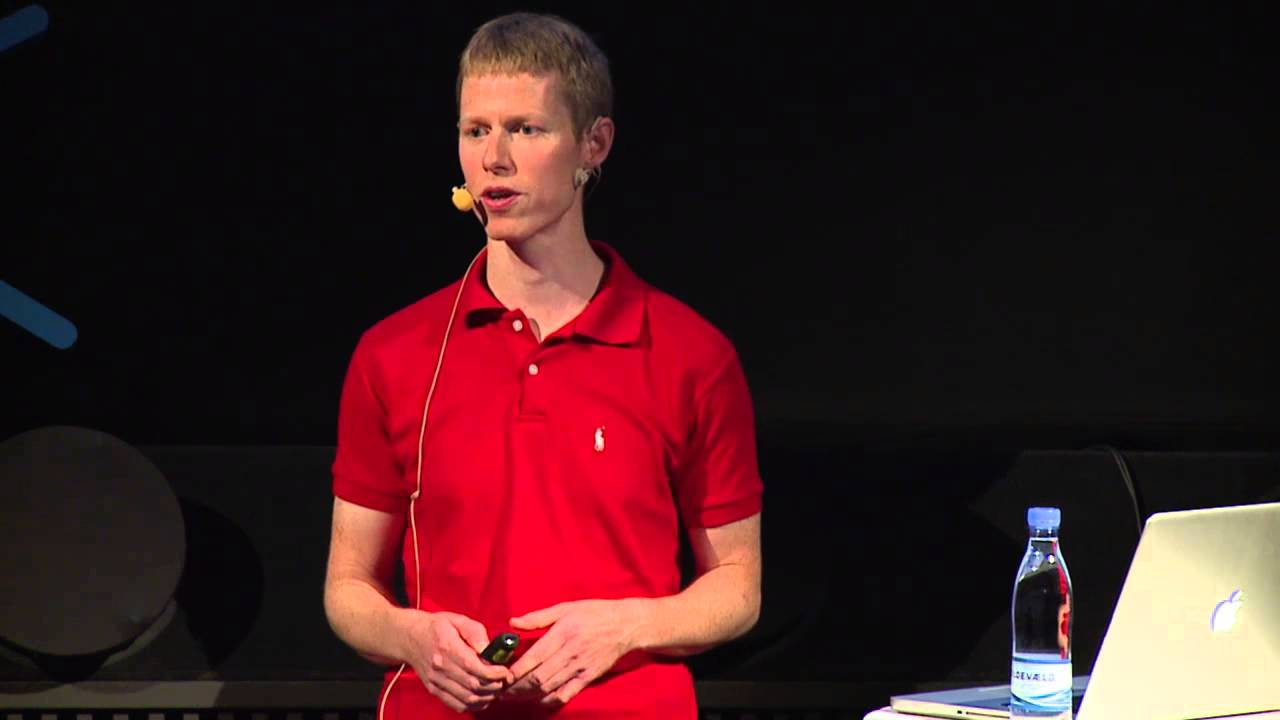
\includegraphics[width=\textwidth,height=3.5cm,keepaspectratio]{Hinhve/KasperLund.jpg}
        \caption{Kasper Lund}
        \label{subfig:kasper_lund}
    \end{subfigure}
    \caption{Các nhà phát triển chính của ngôn ngữ Dart}
    \label{fig:dart_developers}
\end{figure}

\subsection{Lịch sử phát triển của ngôn ngữ lập trình Dart}

Qua hơn một thập kỷ, Dart đã chuyển mình từ một ý tưởng đầy tham vọng thành một ngôn ngữ đa năng, hỗ trợ phát triển ứng dụng trên nhiều nền tảng như web, di động, máy tính để bàn và server. Hành trình trở thành nền tảng phát triển ứng dụng di động hàng đầu của Flutter không dễ dàng mà phải trải qua nhiều tranh chấp pháp lý cũng như những bước tiến vượt bậc về công nghệ. Lịch sử phát triển của Dart có thể được tóm lược qua các giai đoạn chính sau:

\subsubsection{Dart 1.0 (2011 - 2013)}
Dart được công bố lần đầu vào ngày 10 tháng 10 năm 2011 tại hội nghị GOTO ở Aarhus, Đan Mạch. Mục tiêu của Dart là khắc phục các hạn chế của JavaScript, đặc biệt về hiệu suất, khả năng bảo trì mã nguồn, và trải nghiệm lập trình cho các ứng dụng web lớn. 

Tháng 11 năm 2013, Dart 1.0 được phát hành, đánh dấu phiên bản ổn định đầu tiên. Dart 1.0 bao gồm các thành phần chính:

\begin{itemize}
    \item \textbf{Dart Virtual Machine (Dart VM)} cho phép chạy trực tiếp ứng dụng Dart.
    \item \textbf{Trình biên dịch} \texttt{dart2js} để chuyển mã Dart thành JavaScript.
    \item \textbf{Công cụ Dart Editor} hỗ trợ lập trình viên viết mã hiệu quả.
\end{itemize}

Dù được Google hỗ trợ mạnh mẽ, Dart gặp khó khăn trong việc cạnh tranh với JavaScript do sự phổ biến và hệ sinh thái đã phát triển của ngôn ngữ này. Các trình duyệt web phụ thuộc sâu sắc vào JavaScript, khiến Dart khó thay thế như kỳ vọng ban đầu.

\subsubsection{Dart 2.0 (8/2018)}

Tháng 8 năm 2018, Google chính thức giới thiệu \textbf{Dart 2.0}, đánh dấu một bước ngoặt quan trọng trong lịch sử phát triển của ngôn ngữ lập trình này. Phiên bản này không chỉ cải thiện hiệu suất mà còn mang đến những thay đổi nền tảng, giúp Dart trở nên mạnh mẽ và linh hoạt hơn.

    
\textbf{Dart~2.0} đánh dấu bước chuyển quan trọng từ hệ thống kiểu tùy chọn sang hệ thống kiểu tĩnh bắt buộc, củng cố nền tảng \textit{sound static typing} của ngôn ngữ. Bước chuyển này cho phép trình phân tích tĩnh phát hiện lỗi kiểu ngay trong quá trình biên dịch, thay vì đợi tới lúc chạy chương trình. Việc bắt lỗi sớm giúp lập trình viên viết mã an toàn hơn, đồng thời gia tăng độ tin cậy và khả năng dự đoán của ứng dụng, cải thiện hiệu suất và giảm chi phí gỡ lỗi nhờ loại bỏ nhiều lỗi kiểu xuất hiện ở \textit{runtime}. Hệ thống kiểu tĩnh mạnh mẽ cũng khiến \textit{Dart} thu hút những lập trình viên ưa thích \textit{type safety}, đặc biệt là những lập trình viên quen thuộc với ngôn ngữ lập trình \textit{Java} hoặc \textit{C\#} khi có thể tận dụng các công cụ quen thuộc mà vẫn hưởng lợi từ cú pháp gọn nhẹ của \textit{Dart}. Song song với tính nghiêm ngặt, \textit{Dart} vẫn giữ khả năng suy luận kiểu và cho phép dùng từ khóa \textit{dynamic} khi cần sự linh hoạt cao, qua đó cân bằng giữa an toàn và tiện dụng trong phát triển ứng dụng đa nền tảng.









    \textbf{Cải tiến hiệu suất nhờ biên dịch AOT và JIT:} 
    
    Dart 2.0 tận dụng hai phương thức biên dịch mạnh mẽ:

    \begin{itemize}
        \item \textbf{Ahead-of-Time (AOT):} Chuyển mã Dart thành mã máy native trước khi chạy, giúp ứng dụng khởi động nhanh và hoạt động mượt mà, đặc biệt phù hợp với các ứng dụng di động và máy tính để bàn.
        \item \textbf{Just-in-Time (JIT):} Cho phép cập nhật mã nguồn ngay lập tức mà không cần biên dịch lại toàn bộ, hỗ trợ tính năng \textit{hot reload} – một công cụ quan trọng giúp tăng tốc quá trình phát triển ứng dụng.
    \end{itemize}

    \textbf{Định hướng đa nền tảng:} 
    
 Trước đây, \textit{Dart} chủ yếu tập trung vào phát triển web như một lựa chọn thay thế cho \textit{JavaScript}. Sự tập trung đó đã được mở rộng với sự ra đời của \textit{Dart~2.0}, khi \textit{Google} hướng ngôn ngữ này tới cả nền tảng di động và máy tính để bàn. Tầm nhìn mới này đặt nền móng cho \textit{Flutter}, một \textit{framework} đa nền tảng sử dụng \textit{Dart} làm ngôn ngữ chính. Sự xuất hiện của \textit{Flutter} không chỉ mở rộng phạm vi ứng dụng mà còn tái định vị \textit{Dart~2.0} như một ngôn ngữ lập trình đa năng, sẵn sàng cạnh tranh trong nhiều lĩnh vực.









\subsubsection{Sự bùng nổ: Flutter và Dart (2018 - nay)}

Năm 2018, \textit{Google} ra mắt \textit{Flutter}, một \textit{framework} giao diện người dùng (UI) mã nguồn mở cho phép phát triển ứng dụng \textit{native} trên di động, web và máy tính để bàn từ cùng một mã nguồn. \textit{Framework} này chọn \textit{Dart} làm ngôn ngữ lập trình chính, tận dụng những ưu điểm nổi bật của \textit{Dart} để tạo nên một công cụ phát triển mạnh mẽ và hiệu quả.

\begin{itemize}
    \item \textbf{Tính năng \textit{hot reload} giúp tăng tốc phát triển ứng dụng} 
    
    Tính năng \textit{hot reload}, được hỗ trợ bởi biên dịch \textit{JIT} của \textit{Dart}, cho phép nhà phát triển thấy ngay kết quả thay đổi mã nguồn mà không cần khởi động lại ứng dụng. \textit{Hot reload} giúp tiết kiệm thời gian, tăng năng suất và đặc biệt hữu ích trong việc thiết kế, tinh chỉnh giao diện người dùng.
    
    \item \textbf{Biên dịch \textit{native} hiệu quả nhờ AOT kết hợp JIT} 
    
    Cơ chế biên dịch \textit{AOT} của \textit{Dart} tạo mã \textit{native} cho các nền tảng như Android và iOS, bảo đảm hiệu suất cao và trải nghiệm mượt mà, sánh ngang ứng dụng \textit{native} truyền thống. Nhờ đó, \textit{Flutter} có thể cạnh tranh trực tiếp với các công nghệ đa nền tảng như \textit{React Native} hay \textit{Xamarin}.
    
    \item \textbf{Hệ thống \textit{widget} linh hoạt giúp thiết kế giao diện dễ dàng} 
    
    Hệ thống \textit{widget} phong phú cùng cú pháp rõ ràng của \textit{Flutter} cho phép xây dựng giao diện người dùng phức tạp, đẹp mắt mà vẫn đơn giản trong triển khai. Việc dùng một ngôn ngữ duy nhất cho cả logic và giao diện giúp giảm thiểu sự phức tạp khi phải chuyển đổi giữa nhiều ngôn ngữ.
\end{itemize}

Nhờ \textit{Flutter}, \textit{Dart} từ một ngôn ngữ chủ yếu phục vụ lập trình web đã trở thành lựa chọn hàng đầu cho phát triển ứng dụng đa nền tảng. Sự phổ biến của \textit{Flutter} đã thúc đẩy mạnh mẽ việc áp dụng \textit{Dart}, thu hút hàng triệu nhà phát triển trên toàn cầu.


\subsubsection{Dart 2.12: Null Safety (2021)}

Vào tháng 2 năm 2021, \textbf{Dart 2.12} được phát hành, mang đến một trong những tính năng quan trọng nhất trong lịch sử của Dart: \textbf{Null Safety}. Đây là một bước tiến lớn nhằm nâng cao độ an toàn và tin cậy của mã nguồn.

\textit{Null Safety} giúp loại bỏ lỗi \textit{null references}. Tính năng này cho phép lập trình viên chỉ định rõ ràng ngay từ lúc thiết kế liệu một biến có thể nhận giá trị \textit{null} hay không. Sự chỉ định rõ ràng đó ngăn chặn lỗi \textit{null pointer exceptions} – một vấn đề phổ biến và khó chịu trong lập trình. Nhờ phát hiện và xử lý các trường hợp \textit{null} tại thời điểm biên dịch, \textit{Null Safety} nâng cao chất lượng mã, giảm thiểu lỗi \textit{runtime} và cải thiện hiệu suất ứng dụng.


Phiên bản mới này này nhận được sự hoan nghênh nhiệt liệt từ cộng đồng lập trình Dart. \textit{Null Safety} không chỉ giúp mã nguồn trở nên đáng tin cậy hơn mà còn khuyến khích các nhà phát triển viết mã sạch hơn, dễ bảo trì hơn. Đây cũng là minh chứng cho sự trưởng thành của Dart như một ngôn ngữ lập trình hiện đại, đáp ứng các tiêu chuẩn an toàn mã nguồn ngày càng cao.

\subsubsection{Dart 3.x (2023 - 2025)}
Dart tiếp tục phát triển mạnh mẽ với các phiên bản mới, mang đến những tính năng tiên tiến để đáp ứng nhu cầu của các nhà phát triển trong bối cảnh công nghệ không ngừng thay đổi.

\begin{itemize}
    \item \textbf{Dart 3.0 (2023)}: Được phát hành vào năm 2023, Dart 3.0 đánh dấu một cột mốc quan trọng khi yêu cầu tất cả mã nguồn phải tuân thủ Null Safety, đảm bảo tính nhất quán và an toàn trong toàn bộ hệ sinh thái Dart. Ngoài ra, phiên bản này giới thiệu:
    \begin{itemize}
        \item \textbf{Records: } Một cách mới để nhóm các giá trị liên quan mà không cần tạo lớp đầy đủ, giúp mã nguồn gọn gàng và dễ đọc hơn.
        \item \textbf{Patterns: } Hỗ trợ phân tích và so khớp cấu trúc dữ liệu, giúp xử lý dữ liệu phức tạp một cách hiệu quả.
        \item \textbf{Class modifiers: } Cung cấp khả năng kiểm soát tốt hơn việc kế thừa và sử dụng các lớp trong mã nguồn.
    \end{itemize}
    
    \item \textbf{Dart 3.4 (2024)}: Phiên bản này bổ sung hỗ trợ biên dịch sang \textbf{WebAssembly (Wasm)} – một định dạng mã nhị phân cho phép chạy mã với hiệu suất gần native trên trình duyệt. Điều này mở ra tiềm năng lớn cho các ứng dụng Dart trên web, giúp chúng hoạt động nhanh hơn và hiệu quả hơn, cạnh tranh trực tiếp với JavaScript trong các ứng dụng đòi hỏi hiệu suất cao.
    \item \textbf{Dart 3.7 (2025)}: Phiên bản dự kiến ra mắt trong năm 2025. Phiên bản này có những điểm mới:
    \begin{itemize}
        \item \textbf{Wildcard variables:} Cho phép bỏ qua các giá trị không cần thiết trong các biểu thức, giúp mã nguồn ngắn gọn và dễ hiểu hơn.
        \item \textbf{Cải tiến định dạng mã nguồn:} Tăng cường khả năng tự động hóa và chuẩn hóa cách trình bày mã, nâng cao tính nhất quán và dễ bảo trì.
    \end{itemize}
\end{itemize}

\subsection{Ứng dụng thực tiễn của Dart}

Dart ngày càng được ứng dụng rộng rãi, mở rộng ra ngoài phạm vi web và di động, nhờ khả năng thích ứng linh hoạt trên nhiều nền tảng. Khả năng linh hoạt này được thể hiện rõ trong phát triển backend, khi các thư viện như Dart Frog cung cấp giải pháp hiệu quả cho việc xây dựng server-side. Hiệu quả tương tự cũng được khẳng định ở nền tảng web, với Flutter Web và AngularDart hỗ trợ lập trình viên xây dựng ứng dụng giàu tính tương tác từ một cơ sở mã duy nhất. Lợi ích của cơ sở mã duy nhất còn giúp Dart dễ dàng triển khai ứng dụng máy tính để bàn bằng cách biên dịch native trực tiếp cho Windows, macOS và Linux. Không dừng lại ở đó, tính nhỏ gọn và hiệu quả trong biên dịch native còn giúp Dart trở thành lựa chọn lý tưởng cho phát triển các hệ thống IoT và dự án Fuchsia OS.

Sự đa dạng về ứng dụng và tính linh hoạt của Dart được tăng cường hơn nữa nhờ hệ sinh thái Flutter, cho phép lập trình viên phát triển ứng dụng đa nền tảng chất lượng cao chỉ từ một mã nguồn duy nhất, đồng thời hưởng lợi từ quy trình phát triển nhanh và trải nghiệm tinh chỉnh trực quan.



\subsection{Cộng đồng và hệ sinh thái}
Dart hiện sở hữu một cộng đồng phát triển năng động và ngày càng mở rộng. Hệ sinh thái Dart bao gồm hàng loạt thư viện, packages và công cụ hỗ trợ đa dạng, từ phát triển ứng dụng di động với Flutter đến lập trình web và server. Sự hỗ trợ mạnh mẽ từ Google cùng với đóng góp từ cộng đồng đã giúp Dart duy trì vị thế là một ngôn ngữ lập trình quan trọng trong thế giới phần mềm hiện đại.


Hệ sinh thái Dart không ngừng mở rộng, thể hiện ở các hội nghị thường niên quy mô lớn như \textit{Flutter Engage} và \textit{Flutter Forward}, ở công cụ DartPad chạy trực tiếp trên trình duyệt cho phép viết và thực thi mã Dart tức thì, cũng như ở kho gói \texttt{pub.dev} với hàng chục nghìn thư viện mã nguồn mở do cộng đồng đóng góp.









Dart 2.0 giới thiệu hệ thống kiểu tĩnh mạnh mẽ; nền tảng kiểu an toàn này đã mở đường cho sự bùng nổ của Flutter. Sự bùng nổ đó, cùng với \textit{Null Safety} được bổ sung trong Dart 2.12, đã dẫn Dart tiến nhanh tới chuỗi phiên bản 3.x (3.0, 3.4, 3.7) với nhiều cải tiến đáng kể. Quá trình nâng cấp liên tục ấy biến Dart thành một ngôn ngữ đa năng và vững mạnh. Nhờ vậy, theo thống kê năm 2023, Dart đã vươn lên vị trí Top 16 ngôn ngữ lập trình được sử dụng nhiều nhất, khẳng định chỗ đứng vững chắc trong cộng đồng phát triển.


\begin{figure}[H]
    \centering
    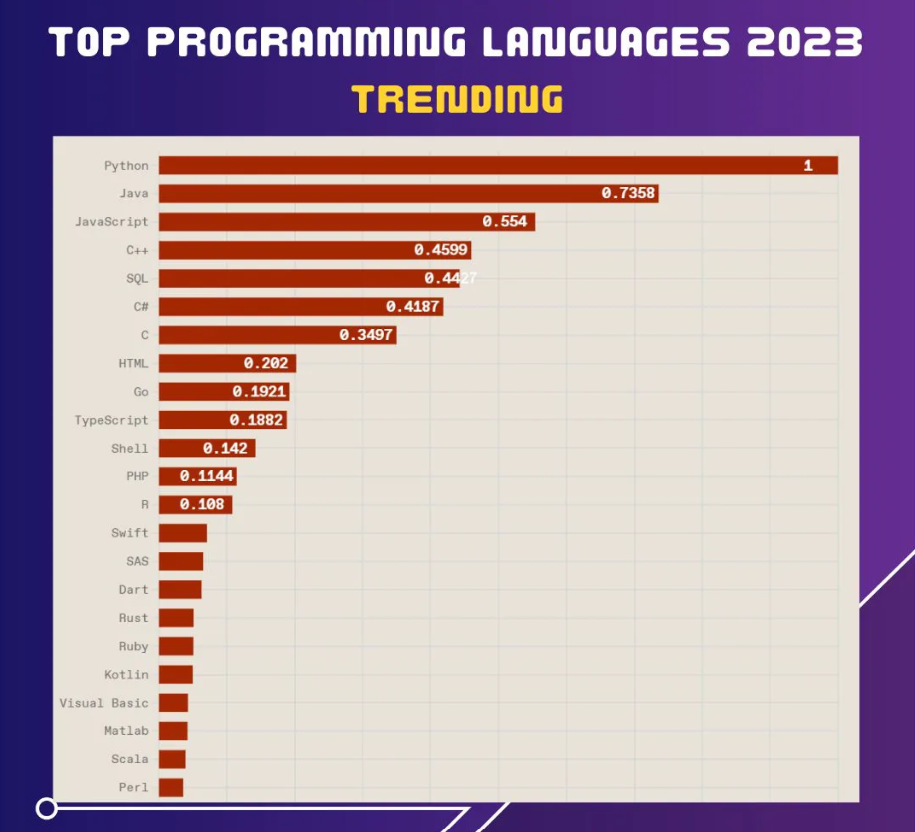
\includegraphics[width=1\textwidth]{Hinhve/ranking.png}
    \caption{Thống kê các ngôn ngữ lập trình phổ biến năm 2023}
    \label{fig:dart_platforms}
\end{figure}

Với vai trò mở rộng trong nhiều lĩnh vực và sự hỗ trợ từ cộng đồng, Dart hứa hẹn sẽ tiếp tục là một công cụ không thể thiếu cho các nhà phát triển trong tương lai.

\section{Đặc điểm của ngôn ngữ lập trình Dart}

\textbf{Dart} là một ngôn ngữ lập trình hiện đại. Ngôn ngữ này chứng tỏ vị thế nổi bật trong phát triển ứng dụng đa nền tảng nhờ khả năng tích hợp chặt chẽ với \emph{Flutter} – framework giao diện người dùng (UI) do Google phát triển. Sự tích hợp đó cho phép \textbf{Dart} tạo ra giao diện mượt mà và hiệu năng cao trên thiết bị di động, trình duyệt web và máy tính để bàn. Ngoài ưu thế tích hợp, cú pháp gần gũi với C, Java và JavaScript giúp lập trình viên đã quen các ngôn ngữ này nhanh chóng nắm bắt cú pháp \textbf{Dart}.

\begin{figure}[H]
    \centering
    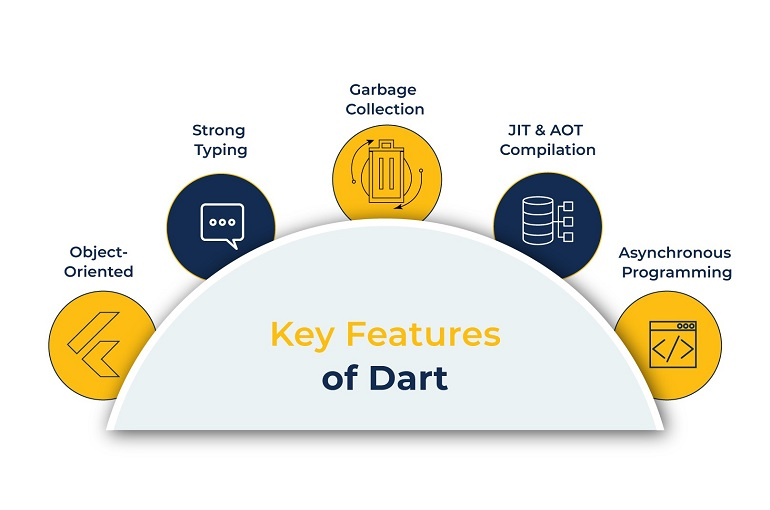
\includegraphics[width=0.7\textwidth]{Hinhve/dartFeatures.jpg}
    \caption{Các đặc điểm chính của ngôn ngữ lập trình Dart}
    \label{fig:dartimg}
\end{figure}

Khả năng thích ứng đa nền tảng tiếp tục được củng cố bởi hệ thống biên dịch linh hoạt của \textbf{Dart}. Cơ chế \emph{ahead-of-time} (AOT) tối ưu hiệu suất thực thi, trong khi \emph{just-in-time} (JIT) hỗ trợ tính năng \emph{hot reload} giúp rút ngắn vòng lặp chỉnh sửa–kiểm thử. Kết hợp với kiểu tĩnh an toàn và bộ thư viện phong phú, tập đặc điểm đó định vị \textbf{Dart} thành lựa chọn lý tưởng cho nhà phát triển đang tìm kiếm một ngôn ngữ duy nhất nhưng đủ mạnh để triển khai ứng dụng trên mọi nền tảng. Những đặc điểm nổi bật dưới đây đã giúp Dart trở thành một lựa chọn lý tưởng cho các nhà phát triển ứng dụng:

\begin{itemize}
\item \textbf{Lập trình bất đồng bộ (Asynchronous Programming):} 
Dart hỗ trợ lập trình bất đồng bộ thông qua các từ khóa \texttt{async} và \texttt{await}, cho phép xử lý các tác vụ không đồng bộ như gọi API, tải dữ liệu, hoặc xử lý sự kiện mà không làm gián đoạn giao diện người dùng. Tính năng này rất quan trọng khi phát triển ứng dụng đa nền tảng, vì nó giúp xây dựng các giao diện động và phản hồi nhanh.Tính năng này giúp Dart trở thành lựa chọn lý tưởng cho các ứng dụng đòi hỏi hiệu suất cao và giao diện mượt mà.

Ví dụ, một hàm bất đồng bộ trong Dart có thể được viết như sau:
    
\begin{lstlisting}
Future<String> fetchData() async {
    await Future.delayed(Duration(seconds: 2));
    return "Loading data successfully!";
}
\end{lstlisting}
    


\item \textbf{Hot Reload:} 
Hot Reload là một trong những tính năng nổi bật nhất khi Dart kết hợp với Flutter, mang lại các tiện ích như :

\begin{itemize}
    \item \textbf{Thay đổi mã nguồn ngay lập tức:} Cho phép lập trình viên thay đổi code và xem ngay kết quả trên giao diện mà không cần khởi động lại toàn bộ ứng dụng.
    \item \textbf{Giữ nguyên trạng thái ứng dụng:} Không làm mất dữ liệu người dùng hoặc trạng thái hiện tại khi reload.
    \item \textbf{Giảm thời gian phát triển:} Giúp tinh chỉnh giao diện UI/UX nhanh chóng, thử nghiệm nhiều phương án chỉ trong vài giây.
    \item \textbf{Ổn định bộ nhớ:} Hạn chế hiện tượng rò rỉ bộ nhớ vốn dễ gặp trong các ngôn ngữ cần build lại toàn bộ như C/C++.
\end{itemize}


\item \textbf{Mã nguồn mở (Open Source):} Dart được phát hành dưới giấy phép BSD-style, nhờ đó cộng đồng lập trình viên toàn cầu có thể trực tiếp tham gia phát triển, báo lỗi và đề xuất cải tiến. Sự tham gia rộng rãi ấy đã hình thành kho thư viện phong phú trên \texttt{pub.dev} với hàng chục nghìn package mã nguồn mở, mở rộng khả năng của Dart trong hầu hết các lĩnh vực. Kho thư viện không ngừng lớn mạnh tiếp tục thúc đẩy nhu cầu về tư liệu học tập; tài liệu chính thức tại \texttt{dart.dev} và \texttt{flutter.dev} vì thế luôn được cập nhật thường xuyên, hỗ trợ đồng thời người mới bắt đầu và lập trình viên chuyên nghiệp. Việc tài liệu và thư viện phát triển liên tục góp phần mở rộng hệ sinh thái dựa trên Dart: từ Flutter và AngularDart đến các giải pháp server-side như Shelf hay Dart Frog. Môi trường mã nguồn mở toàn diện như vậy đã thúc đẩy sự phát triển nhanh chóng và bền vững của Dart kể từ khi ra đời.









\vspace{0.5cm}

\item \textbf{Kiểu tĩnh (Statically Typing):} 
Dart sử dụng hệ thống kiểu dữ liệu tĩnh với thiết kế âm thanh (sound type system), giúp:

\begin{itemize}
    \item \textbf{Phát hiện lỗi sớm:} Kiểm tra kiểu dữ liệu ngay tại thời điểm biên dịch, giảm thiểu lỗi runtime.
    \item \textbf{Cải thiện độ an toàn:} Bắt lỗi kiểu dữ liệu hoặc thiếu Null Safety ngay khi lập trình, trước khi ứng dụng được chạy thực tế.
    \item \textbf{Hỗ trợ Null Safety (từ Dart 2.12):}
    \begin{itemize}
        \item Các biến phải khai báo rõ ràng nếu có thể nhận giá trị \texttt{null} (ví dụ: \texttt{int? value;}).
        \item Loại bỏ hoàn toàn lỗi phổ biến \texttt{NullPointerException}.
    \end{itemize}
    \item \textbf{Giữ cú pháp ngắn gọn:} Với cơ chế suy luận kiểu (type inference), Dart cho phép viết mã ngắn mà vẫn đảm bảo an toàn:
    \begin{verbatim}
    var name = 'Dart'; // kiểu String
    \end{verbatim}
\end{itemize}

Hệ thống kiểu của Dart mang lại sự cân bằng tuyệt vời giữa hiệu suất, độ an toàn và trải nghiệm lập trình linh hoạt.

    \item \textbf{Tính di động (Portability):} 
Dart được thiết kế để trở thành ngôn ngữ \textbf{"write once, run anywhere"}, cho phép biên dịch mã nguồn sang nhiều nền tảng khác nhau mà không cần thay đổi logic chính.
\begin{itemize}
\item \textbf{Native code (AOT):} Cơ chế \textit{ahead-of-time compilation} của Dart biên dịch trực tiếp mã nguồn sang mã máy ARM hoặc~x86. Cấu trúc biên dịch ấy cho phép tạo các gói cài đặt \textit{APK}, \textit{IPA} hay tệp \textit{EXE} cho ứng dụng Flutter trên di động và máy tính để bàn, đồng thời bảo đảm hiệu suất native và thời gian khởi chạy nhanh.

\item \textbf{JavaScript (dart2js):} Trình biên dịch \textit{dart2js} chuyển đổi mã Dart sang JavaScript được tối ưu cho trình duyệt. Quy trình này áp dụng kỹ thuật \textit{tree-shaking} nhằm loại bỏ mã thừa, giảm kích thước tệp sinh ra và đạt hiệu suất cao hơn khoảng 20 \% so với JavaScript viết tay trong các phép đo chuẩn.

\item \textbf{WebAssembly (từ Dart 3.4):} Kể từ phiên bản 3.4, Dart hỗ trợ biên dịch sang \textit{WebAssembly} thông qua phần mở rộng \textit{WasmGC}. Cách biên dịch này nâng hiệu suất tải và thực thi ứng dụng web thêm 30–50 \% so với JavaScript.

\item \textbf{Server-side và file thực thi độc lập:} Trong giai đoạn phát triển, mã Dart có thể chạy trực tiếp trên \textit{Dart VM}; khi triển khai, cùng một mã nguồn ấy được biên dịch thành tệp thực thi độc lập cho môi trường sản xuất. Ví dụ tiêu biểu là hạ tầng Google Fiber đã dùng Dart ở server-side để xử lý khoảng 10 000 yêu cầu mỗi giây.

\item \textbf{Casestudy đa nền tảng:} Ứng dụng Google Ads minh họa rõ ràng tính “write once, run anywhere”: một codebase Dart duy nhất phục vụ đồng thời năm nền tảng—Android, iOS, web, Windows và macOS—giúp rút ngắn ước tính 70 \% thời gian phát triển so với duy trì năm dự án riêng rẽ.
\end{itemize}

    \item \textbf{Công cụ hỗ trợ mạnh mẽ (Productive Tooling):} 
    Dart đi kèm với các công cụ phát triển mạnh mẽ, bao gồm DartPad (một trình biên tập trực tuyến cho phép viết và chạy mã Dart mà không cần cài đặt), và tích hợp tốt với các IDE như Visual Studio Code, IntelliJ IDEA, và Android Studio. Các công cụ này cung cấp tính năng gợi ý mã, kiểm tra lỗi thời gian thực, và gỡ lỗi, giúp tăng năng suất lập trình. Ngoài ra, Dart còn có hệ thống quản lý gói (package manager) gọi là \texttt{pub}, giúp dễ dàng quản lý và tích hợp các thư viện bên ngoài.

    \item \textbf{Thu gom rác (Garbage Collection):} 
        Dart có hệ thống quản lý bộ nhớ tự động thông qua thu gom rác, giúp giảm thiểu lỗi liên quan đến bộ nhớ như rò rỉ bộ nhớ (memory leak). Hệ thống này tự động giải phóng bộ nhớ không còn sử dụng, đảm bảo hiệu suất ổn định cho ứng dụng, đặc biệt là các ứng dụng lớn và phức tạp.
        Theo bài kiểm tra của Google, Dart GC giảm 50\% thời gian tạm dừng so với JavaScript V8 trong các ứng dụng phức tạp.

    \item \textbf{Nền tảng cho Flutter:} 
    Dart là ngôn ngữ chính thức của Flutter, một framework của Google để xây dựng ứng dụng giao diện người dùng đa nền tảng. Sự kết hợp giữa Dart và Flutter mang lại hiệu suất cao nhờ biên dịch AOT, cùng với khả năng tạo giao diện đẹp mắt và đồng nhất trên các nền tảng. Tính năng Hot Reload và lập trình bất đồng bộ của Dart đặc biệt hữu ích trong Flutter, giúp lập trình viên phát triển ứng dụng nhanh chóng và hiệu quả.

    \item \textbf{Hỗ trợ lập trình hướng đối tượng (Object-Oriented Programming):} 
    Dart là một ngôn ngữ hướng đối tượng hoàn chỉnh, hỗ trợ các khái niệm như lớp, giao diện, mixin, và lớp trừu tượng. Điều này cho phép lập trình viên xây dựng các ứng dụng có cấu trúc rõ ràng và dễ bảo trì.
\end{itemize}
Lựa chọn ngôn ngữ lập trình phù hợp là yếu tố then chốt bảo đảm hiệu suất và khả năng mở rộng của ứng dụng. Sự lựa chọn này thường được cân nhắc giữa hai ngôn ngữ phổ biến là Dart và JavaScript, mỗi ngôn ngữ sở hữu những đặc điểm riêng. Các đặc điểm ấy sẽ được trình bày trong Bảng so sánh các tiêu chí giữa Dart và JavaScript như sau:
















\begin{table}[H]
\centering
\begin{tabular}{|>{\centering\arraybackslash}p{4.5cm}|>{\centering\arraybackslash}p{4.5cm}|>{\centering\arraybackslash}p{4.5cm}|}
\hline
\textbf{Tiêu chí} & \textbf{Dart} & \textbf{JavaScript} \\ \hline
Kiểu dữ liệu & Kiểu tĩnh (Statically Typed), hỗ trợ Null Safety & Kiểu động (Dynamically Typed) \\ \hline
Thu gom rác & Bộ thu gom rác thế hệ (Generational GC) & Bộ thu gom rác incremental truyền thống \\ \hline
Biên dịch & AOT và JIT compilation, hỗ trợ native & Chạy trực tiếp trên trình duyệt (interpreted) \\ \hline
Công cụ hỗ trợ & DartPad, Flutter DevTools, Analyzer & Chrome DevTools, VSCode, Node.js Tools \\ \hline
Tính di động & Web, mobile, desktop, server, IoT, Fuchsia OS & Web, server (Node.js) \\ \hline
Hiệu suất & Native tốc độ cao với AOT, nhanh hơn trong mobile apps & Tối ưu tốt trên trình duyệt, nhưng mobile native chậm hơn Dart+Flutter \\ \hline
\end{tabular}
\caption{Bảng so sánh các đặc điểm giữa Dart và JavaScript}
\label{tab:dart_vs_js}
\end{table}

\section{Các nền tảng thực thi của Dart}

Dart hỗ trợ hai nền tảng chính cho việc phát triển ứng dụng: \textbf{Dart Native} và \textbf{Dart Web}. Như được minh họa trong \textit{Hình \ref{fig:dart_platforms}}, mỗi nền tảng có các đặc điểm và mục đích sử dụng riêng biệt, cho phép các nhà phát triển xây dựng ứng dụng đa nền tảng một cách hiệu quả.

\begin{figure}[H]
    \centering
    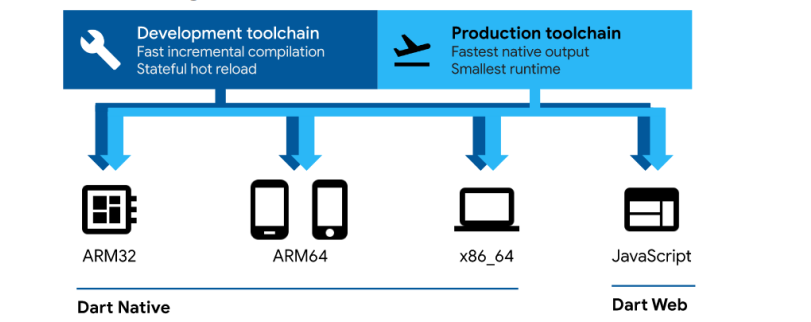
\includegraphics[width=1\textwidth]{Hinhve/dartPlatform.png}
    \caption{Các nền tảng thực thi của Dart}
    \label{fig:dart_platforms}
\end{figure}

\subsection{Dart Native}

Dart Native được thiết kế để phát triển ứng dụng di động và máy tính để bàn. Nó cho phép biên dịch mã Dart thành mã máy bản xứ, đảm bảo hiệu suất cao trên các nền tảng như Android, iOS, Windows, macOS, và Linux. Dart Native hỗ trợ các kiến trúc phần cứng như ARM32, ARM64 (cho thiết bị di động) và x86\_64 (cho máy tính để bàn).

Trong quá trình phát triển, Dart Native cung cấp:
\begin{itemize}
    \item \textbf{Biên dịch tăng cường nhanh chóng}: Giúp lập trình viên thấy ngay kết quả thay đổi mã mà không cần khởi động lại ứng dụng.
    \item \textbf{Hot reload}: Cho phép cập nhật mã nguồn trong thời gian thực, giữ nguyên trạng thái ứng dụng, rất hữu ích cho thiết kế giao diện.
\end{itemize}



\subsection{Dart Web}

Dart Web cho phép phát triển ứng dụng web bằng cách biên dịch mã Dart thành JavaScript, cho phép chạy trên bất kỳ trình duyệt web hiện đại nào. Điều này giúp xây dựng ứng dụng web phức tạp với hiệu suất cao, tận dụng các tính năng như hệ thống kiểu dữ liệu tĩnh và lập trình bất đồng bộ.

Từ phiên bản 3.4, Dart Web còn hỗ trợ biên dịch sang WebAssembly, tăng hiệu suất thêm 30-50\% so với JavaScript, đặc biệt cho ứng dụng web không dùng Flutter.

\section{Cộng cụ phát triển ứng dụng trên Dart}

Dart SDK cung cấp một bộ công cụ mạnh mẽ để hỗ trợ phát triển ứng dụng trên nhiều nền tảng. Dưới đây là các công cụ chính và cách sử dụng của chúng:

\subsection{Công cụ chính của Dart SDK}

\begin{itemize}
    \item \textbf{dart}: Giao diện dòng lệnh để tạo, chạy, phân tích, kiểm tra, biên dịch và đóng gói Dart.
    \begin{itemize}
        \item \textbf{dart run}: Chạy các chương trình Dart.
        \item \textbf{dart analyze}: Phân tích mã nguồn để tìm lỗi và cảnh báo.
        \item \textbf{dart test}: Chạy các bài kiểm tra đơn vị.
        \item \textbf{dart compile}: Biên dịch Dart thành các định dạng khác nhau:
        \begin{itemize}
            \item \textbf{exe}: Tạo ra một tệp thực thi độc lập cho Windows, macOS, hoặc Linux, bao gồm mã đã biên dịch và một runtime Dart nhỏ.
            \item \textbf{aot-snapshot}: Tạo ra một module AOT đã biên dịch, phụ thuộc vào kiến trúc phần cứng, không bao gồm runtime Dart.
            \item \textbf{jit-snapshot}: Tạo ra một module JIT với các lớp đã phân tích và mã đã biên dịch từ một lần chạy huấn luyện, giúp khởi động nhanh hơn.
            \item \textbf{kernel}: Đóng gói ứng dụng vào một tệp portable chứa Kernel AST, có thể chạy trên tất cả các hệ điều hành và kiến trúc CPU.
            \item \textbf{js}: Biên dịch Dart thành JavaScript có thể triển khai, với các mức tối ưu hóa từ -O0 đến -O4.
            \item \textbf{wasm}: Biên dịch thành WebAssembly (đang trong giai đoạn phát triển).
        \end{itemize}
    \end{itemize}
    \item \textbf{dartdoc}: Trình tạo tài liệu, giúp tạo ra tài liệu tham khảo HTML từ mã nguồn Dart.
    \begin{itemize}
        \item Sử dụng: Chạy lệnh \texttt{dart doc .} trong thư mục gốc của gói sau khi chạy \texttt{dart pub get}.
        \item Kết quả: Tài liệu được đặt trong thư mục \texttt{doc/api} (có thể cấu hình).
    \end{itemize}
    \item \textbf{pub}: Trình quản lý gói, cho phép quản lý các gói phụ thuộc cho dự án Dart.
    \begin{itemize}
        \item \textbf{pub get}: Lấy các gói phụ thuộc được chỉ định trong tệp \texttt{pubspec.yaml}.
        \item \textbf{pub upgrade}: Nâng cấp các gói phụ thuộc lên phiên bản mới nhất phù hợp với ràng buộc trong \texttt{pubspec.yaml}.
        \item \textbf{pub publish}: Đăng gói lên pub.dev để người khác có thể sử dụng.
        \item \textbf{pub global activate}: Làm cho các công cụ dòng lệnh của gói có sẵn toàn cục.
    \end{itemize}
\end{itemize}

\subsection{Công cụ cho phát triển web}

Để phát triển các ứng dụng trên nền web, Dart cung cấp các công cụ sau:

\begin{itemize}
    \item \textbf{dart2js}: Biên dịch Dart thành JavaScript, cho phép chạy ứng dụng Dart trên trình duyệt web.
    \begin{itemize}
        \item Sử dụng: Chạy lệnh \texttt{dart compile js} (thay thế cho \texttt{dart2js} trong các phiên bản cũ).
        \item Tùy chọn: Có thể tối ưu hóa với các cờ như -O0 đến -O4.
    \end{itemize}
    \item \textbf{webdev}: Công cụ dòng lệnh để biên dịch và kiểm tra ứng dụng web Dart.
    \begin{itemize}
        \item \textbf{serve}: Khởi động máy chủ phát triển để gỡ lỗi với các cập nhật tăng cường (hot reload).
        \item \textbf{build}: Tạo ra mã JavaScript đã tối ưu hóa cho sản xuất.
    \end{itemize}
    \item \textbf{dartdevc}: Biên dịch phát triển Dart thành JavaScript (cho môi trường phát triển), hỗ trợ biên dịch modular nhanh chóng cho các trình duyệt hiện đại.
    \begin{itemize}
        \item Sử dụng: Tự động được sử dụng khi chạy \texttt{webdev serve} trong chế độ phát triển.
    \end{itemize}
\end{itemize}

Các công cụ trên không chỉ hỗ trợ phát triển ứng dụng Dart mà còn giúp tối ưu hóa quy trình làm việc, từ việc quản lý phụ thuộc đến biên dịch và triển khai. Đặc biệt, với sự kết hợp của Flutter, Dart đã trở thành một ngôn ngữ mạnh mẽ cho phát triển ứng dụng đa nền tảng. Các công cụ như \texttt{webdev} và \texttt{dartdevc} giúp phát triển web nhanh chóng và hiệu quả, trong khi \texttt{dart compile} và \texttt{pub} đảm bảo tính linh hoạt và khả năng mở rộng của các dự án.

\section{Chương trình minh họa}
Dưới đây là một ví dụ mẫu về một chương trình minh họa sử dụng ngôn ngữ lập trình Dart.

\textit{Ví dụ:}
\begin{lstlisting}
// First Programming
void main() {
    var a = 'World';
    print('Hello $a');
} 
\end{lstlisting}

\begin{itemize}
    \item \textbf{Hàm \texttt{main()}}: Đây là điểm bắt đầu của mọi chương trình Dart. Khi chương trình được thực thi, Dart runtime sẽ tìm và chạy hàm \texttt{main()} đầu tiên. Nếu không có hàm \texttt{main()}, chương trình sẽ không thể chạy được và sẽ báo lỗi.
    
    \item \textbf{Từ khóa \texttt{void}}: Từ khóa này chỉ ra rằng hàm \texttt{main} không trả về giá trị nào. Dart yêu cầu rõ ràng về kiểu dữ liệu của hàm để đảm bảo tính an toàn kiểu (type safety).
    
    \item \textbf{Câu lệnh \texttt{var a = 'World';}}: 
    \begin{itemize}
        \item Từ khóa \texttt{var} cho phép khai báo biến mà không cần chỉ định kiểu dữ liệu tường minh; Dart sẽ tự động suy luận kiểu dựa trên giá trị được gán.
        \item Trong ví dụ trên, \texttt{a} sẽ được xác định là kiểu \texttt{String} vì nó được gán giá trị chuỗi \texttt{'World'}.
    \end{itemize}
    
    \item \textbf{Câu lệnh \texttt{print('Hello \$a');}}:
    \begin{itemize}
        \item Hàm \texttt{print()} được sử dụng để in dữ liệu ra màn hình console.
        \item Cú pháp \texttt{\$a} trong chuỗi là cách nội suy biến (string interpolation) trong Dart, cho phép chèn giá trị biến \texttt{a} trực tiếp vào chuỗi mà không cần phép nối thủ công.
    \end{itemize}
\end{itemize}

\textbf{Thực thi chương trình:} 

Để chạy chương trình Dart đơn giản này, ta thực hiện các bước sau:
\begin{enumerate}
    \item Lưu đoạn mã vào một file với phần mở rộng \texttt{.dart}, ví dụ: \texttt{hello\_world.dart}.
    \item Mở terminal hoặc command prompt, chuyển đến thư mục chứa file đó.
    \item Gõ lệnh:
    \begin{verbatim}
    dart hello_world.dart
    \end{verbatim}
    \item Nếu mọi thứ đúng, ở terminal sẽ hiển thị kết quả:
    \begin{verbatim}
    Hello World
    \end{verbatim}
\end{enumerate}

\textbf{Giới thiệu công cụ DartPad:} 

Dưới đây là hình ảnh của công cụ DartPad trong thực tế với 1 Project minh họa nhỏ về game TicTacToe:

\begin{figure}[H]
    \centering
    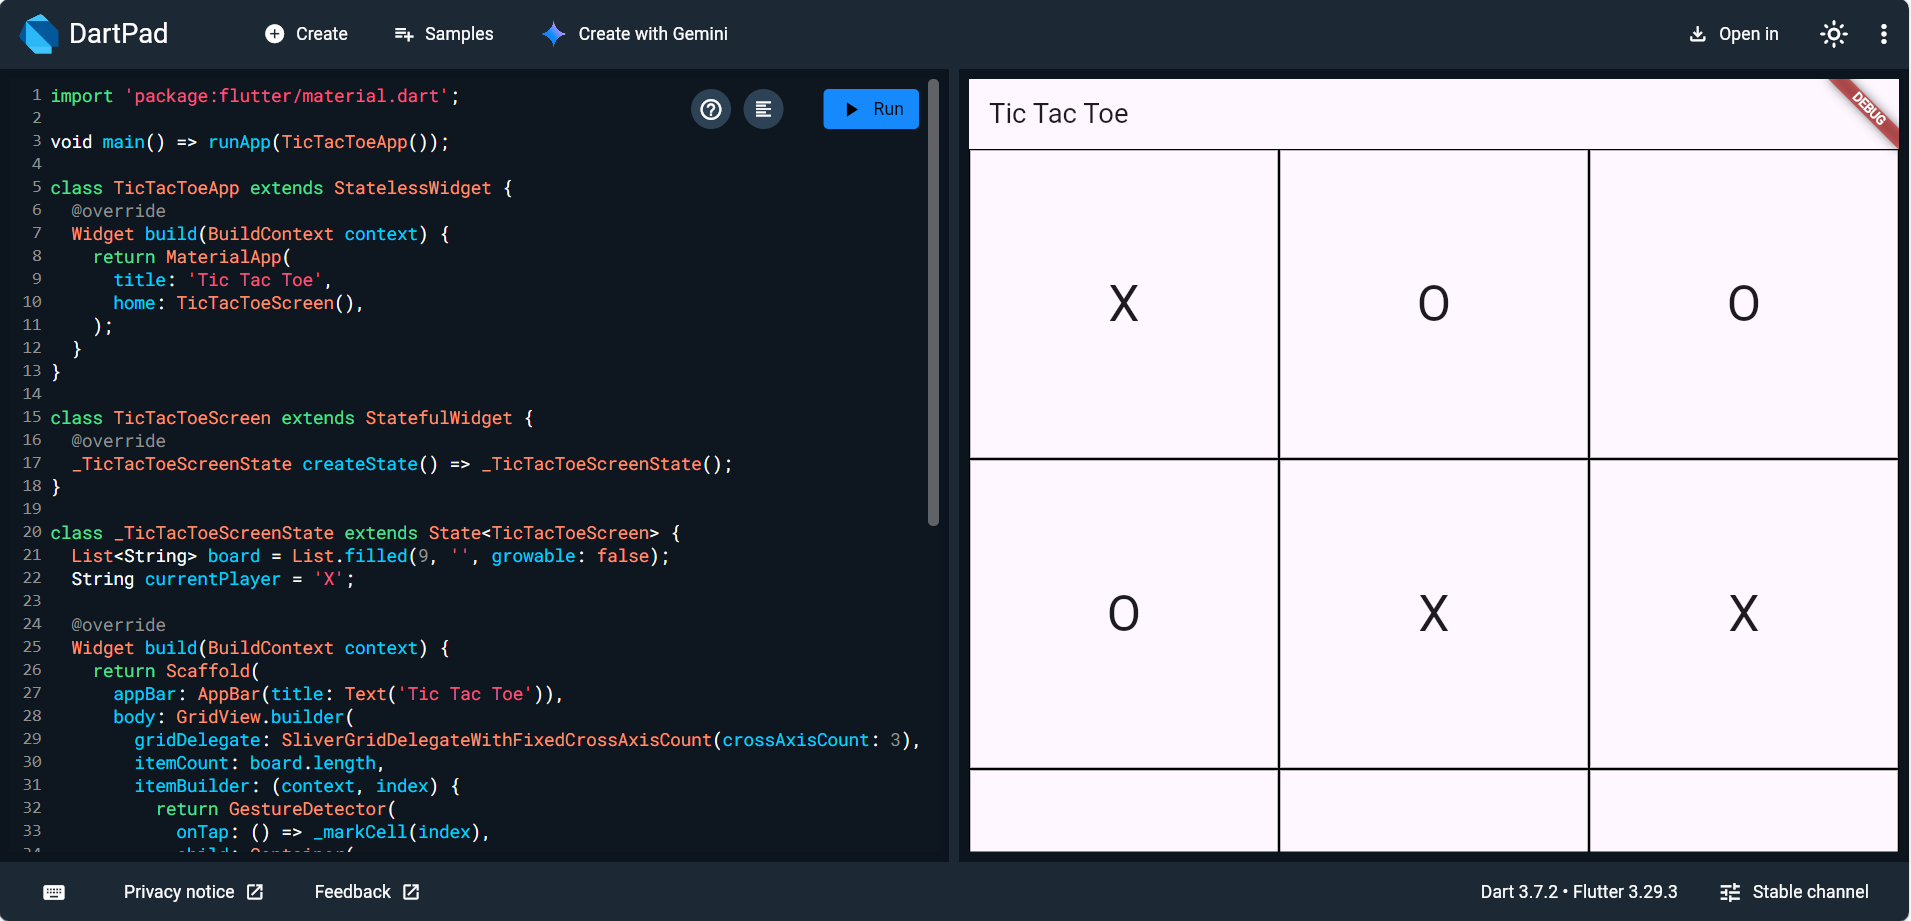
\includegraphics[width=1\textwidth]{Hinhve/dartpad.png}
    \caption{Công cụ Dartpad}
    \label{fig:dartimg}
\end{figure}


\textbf{DartPad} là một công cụ cực kỳ hữu ích do Google cung cấp, cho phép người học và lập trình viên thử nghiệm và thực thi mã Dart ngay trên trình duyệt mà không cần cài đặt bất kỳ phần mềm nào .

\begin{itemize}
    \item Truy cập DartPad tại địa chỉ: \url{https://dartpad.dev/}
    \item DartPad hỗ trợ đầy đủ cú pháp Dart, tính năng kiểm tra lỗi thời gian thực, và thậm chí còn hỗ trợ lập trình Flutter để phát triển giao diện người dùng ngay trong trình duyệt.
    \item Người dùng có thể:
    \begin{itemize}
        \item Viết mã Dart nhanh chóng và dễ dàng.
        \item Thực thi chương trình và xem kết quả ngay lập tức.
        \item Chia sẻ đoạn mã của mình qua URL ngắn gọn.
    \end{itemize}
    \item DartPad rất hữu ích cho:
    \begin{itemize}
        \item Sinh viên mới học lập trình.
        \item Người dạy học hoặc thuyết trình giới thiệu về Dart/Flutter.
        \item Lập trình viên muốn kiểm tra nhanh một đoạn mã nhỏ.
    \end{itemize}
\end{itemize}

\end{document}
